\documentclass[a4paper]{article}
\usepackage[utf8]{inputenc}
\usepackage{amsfonts}
\usepackage{amsmath}
\usepackage{amsthm}
\usepackage{graphicx}
\usepackage{array}
\usepackage[footnotesize,bf,format=hang]{caption}
\usepackage{mathtools}
\usepackage{booktabs}
\usepackage{subfigure}
\usepackage{textcomp} % For the cent symbol
%\usepackage[font=footnotesize]{subcaption}
\usepackage{varioref}
\captionsetup{justification=justified, singlelinecheck=true}
\usepackage[backend=biber,url=false,doi=true,style=authoryear]{biblatex}
\addbibresource{library.bib}
\usepackage{authblk}
\usepackage{attrib}
\usepackage{enumerate}
%\bibliographystyle{elsarticle-harv}
\usepackage{cleveref}
%\nocite{*}
% % Diagramming
\usepackage{tikz}
\usepackage{float}
\usetikzlibrary{arrows,positioning,decorations}
% %

\title{A global inter-country economic model based on linked input-output models}
\author[*]{Robert G. Levy}
\author[**]{Thomas P. Ol\'{e}ron Evans}
\author[*]{Alan G. Wilson}

\affil[*]{Centre for Advanced Spatial Analysis, UCL Bartlett Faculty of the Built Environment,
90 Tottenham Court Road, London W1T 4TJ, UK}
\affil[**]{Department of Mathematics, University College London, Gower Street, London WC1E 6BT, UK}


\begin{document}
\maketitle

\begin{abstract}
We present a new, flexible and extensible alternative to multi-regional input-output (MRIO) for modelling the global economy.
The limited coefficient set of MRIO (technical coefficients only) is extended to include two new sets of coefficients, import ratios and import propensities.
These new coefficient sets assist in the interaction of the new model with other social science models such as those of trade, migration, international security and development aid.
The model uses input-output models as descriptions of the internal workings of countries' economies, and couples these more loosely than in MRIO using trade data for commodities and services from the UN.
The model is constructed using a minimal number of assumptions, seeks to be as parsimonious as possible in terms of the number of coefficients, and is based to a great extent on empirical observation.
Two new metrics are introduced, measuring sectors' economic significance and economic self-reliance per country.
The Chinese vehicles sector is shown to be the world's most significant, and self-reliance is shown to be strongly correlated with population.
The new model is shown to be equivalent to an MRIO under an additional assumption, allowing existing analysis techniques to be applied.
\end{abstract}

\section{Introduction}
The objective of this paper is to present a global economic model that can be used as the basis for assessing the impacts of future changes in trade, migration, security and development aid.
Because these topics are often associated with developing countries, it is important that the model have as few coefficients as possible, to enable the future addition of countries who publish little data on their economic structure.
The model as it is presented here represents a first `proof of concept' step towards these ambitious goals.
At this stage, the focus is on creating a model of global trade which will form a skeleton onto which additional social science models will be added in future work.
The economies of individual countries are represented as 35-sector input-output models, each of which is linked through trade flows representing imports and exports.
This has recently been made feasible by the publication of the World Input-Output Database (WIOD) \parencite{timmer_world_2012}, a collection of national input-output tables (NIOTs) for 40 (mostly developed) countries across 17 years, from 1995 to 2011.
The NIOTs are linked through data from the UN, covering trade in both products\footnote{comtrade.un.org/db} and services\footnote{unstats.un.org/unsd/servicetrade/}.

While other models of world trade based on the input-output methodology exist, the model presented here is one of the first to integrate the extremely detailed internal economic data provided by WIOD with the enormous wealth of trade data from the UN COMTRADE database, resulting in a picture of global trade that includes an unparalleled amount of empirically derived economic information.
The use of such data sources and the simplicity and flexibility of the model proposed will allow for the investigation of a of wide range of economic scenarios, including those involving developing countries, in future work.

The remainder of this paper is structured as follows: 
Section \ref{sec:litreview} gives an overview of existing work in this area;
Section \ref{sec:system} gives a description of the present system and outlines how data is used to calibrate the coefficients of the model;
The algorithm used to calculate the output of the model is described in section \ref{sec:algorithm} and some preliminary results are given in section \ref{sec:analysis}.
Conclusions and potential directions for future research are presented in section \ref{sec:conclusions}.

\section{Existing global economic models} \label{sec:litreview}
In the mid-1970s, the creator of input-output economics, Wassily Leontief, used the acceptance speech of his Nobel prize in Economics to announce a very ambitious project to model the global economy:

\begin{quotation}
Major efforts are underway to construct a data base for a systematic input-output study not of a single national economy but of the world economy viewed as a system composed of many interrelated parts [...]
Preliminary plans provide for a description of the world economy in terms of twenty-eight groups of countries, with about forty-five productive sectors for each group. \attrib{\cite{leontief_structure_1974}}
\end{quotation}

\textcite{duchin_international_2004} describes how, twenty years on, Leontief's efforts in this area had largely been ignored by economists who describe his departures from the standard, neoclassical modelling in terms of price elasticity and elasticity of substitution as being ``too great to ignore''. 
See section \ref{sec:iots} for more on this subject.

In the years since Leontief published his global model, input-output analysis has been largely restricted to regional studies, of which \textcite{akita_interregional_1993}, \textcite{khan_sectoral_1999} and \textcite{luo_power--pull_2013} are examples; and studies related to energy and the environment, such as  \textcite{leontief_environmental_1970}, \textcite{joshi_product_1999}, \textcite{bergh_handbook_2002} and \textcite{hendrickson_environmental_2006}.

However, much more recently, attention has returned to input-output modelling in a global context more generally. \textcite{tukker_global_2013} describe how several multi-regional input-output (MRIO) models have been developed in the very recent literature.
These are, along with WIOD which is used in the present model, EORA \parencite{lenzen_building_2013}, EXIOPOL \parencite{tukker_exiopol_2013} and the more mature GTAP \parencite{walmsley_introduction_2012}.

Each of these existing models of the global economy extends the idea of the national input-output table to an international setting: where in a NIOT the magnitude of every bilateral sector--sector flow is recorded for a given country, these projects record the magnitude of every country/sector--country/sector flow.
Thus, for example, the extent to which British agriculture purchases from Belgian manufacturing is recorded in dollar amounts.
This results in a large matrix which, through inversion in the normal input-output fashion, can be used to predict the impact of a particular exogenous change in demand.
This tends to strengthen the case of those economists, mentioned by \textcite{duchin_international_2004}, that price- and substition-elasticities are ignored by input-output economics.

The model presented in this paper provides a framework in which the power of input-output analysis at the national level can be combined with a more subtle understanding of the dynamics of international trade.
The standard MRIO of $C$ countries and $S$ sectors requires $SC\times SC$ coefficients and a major goal of this model is to minimise the number of coefficients required to model a global system.
It also provides modellers with a richer set of coefficients than the standard technical coefficients of MRIOs in order to facilitate the combination of the present model with other models of human systems, such as migration, international security and development aid. 
Additionally, as mentioned, this reduced set of coefficients will facilitate the addition of countries vital to the study of these systems, but which do not publish data on economics structure.
The mathematical estimation of the coefficients for these countries is the subject of upcoming work.

\section{Description of the model} \label{sec:system}
Here we outline the new global model.
In this presentation the model has $C$ countries, the economies of which are divided into $S$ productive sectors\footnote{Although each sector produces many distinct products, for the sake of simplicity, these products are considered to be perfect substitutes, allowing the terms `sector' and `product' to be used interchangeably throughout this paper.}.
All product flows are given by value, measured in millions of (current price) US dollars\footnote{This allows us to use the terms `quantity' and `value' interchangeably.}.
We start with an introduction to input-output tables which, aside from some important notation, can be skipped by the reader familiar with this topic.
We then introduce the model of a single country, and outline both the normal input-output coefficient sets and introduce the first new set.
Finally we show how these country models are linked with an international trade model and introduce the second new set of coefficients.
%The following rows of the NIOTs are combined into a single `Value Added' flow source (not completely equivalent to ``Value added at basic prices", used in WIOD), which represents the total value of products produced by each sector after the subtraction of the sum of its intermediate demands on other sectors:
%\begin{enumerate}
%\itemsep -0.4em 
%\item Taxes less subsidies on products
%\item CIF/FOB adjustments on exports
%\item Direct purchases abroad by residents
%\item Purchases on the domestic territory by non-residents
%\item Value added at basic prices
%\item International transport margins
%\end{enumerate}
%Although `Value Added' is not used in the current iteration of the model, it provides a loose measure of `profitability' or `efficiency' for each sector that may prove useful in future applications and extensions.

\subsection{Introduction to input-output tables} \label{sec:iots}
Input-output is, at its heart, an accounting methodology.
The products produced by and imported into a given country in a given year are either: sold as inputs to other sectors (`intermediate supply'); supplied to the `final demand' of consumers and the government; invested; or exported.
The total amount imported and produced must equal the amount used, consumed, invested and exported for each sector.

By simple summation, country $i$'s total production of sector $s$, $x_s^{(i)}$, can be defined as the sum of all intermediate supply, plus supply to final demand, investment and export:

\begin{equation}\label{eqn:x}
x_s^{(i)}=\sum\limits_{t}z_{s,t}^{\dagger(i)} + f_s^{\dagger(i)} + n_s^{\dagger(i)} + e_s^{(i)}
\end{equation}
where $z_{s,t}^{\dagger(i)}$ is the intermediate supply from domestic sector $s$ to sector $t$ in country $i$, $f_s^{\dagger(i)}$ is final demand for domestic sector $s$, $n_s^{\dagger(i)}$ is investment and $e_s^{(i)}$ are exports.

Similarly, country $i$'s total import of sector $s$, $m_s^{(i)}$, is the sum of all intermediate supply of imported products, plus demand for and investment of imported products\footnote{
Note that, by convention, imported products may not be directly exported.
This is a convention we retain throughout.
}:

\begin{equation}\label{eqn:m}
m_s^{(i)}=\sum\limits_{t}z_{s,t}^{*(i)} + f_s^{*(i)} + n_s^{*(i)}
\end{equation}
An input-output table, $\boldsymbol{T}^{(i)}$, as described by \textcite{miller_input-output_1985}, is a particular arrangement of these quantities, which provides a clear and compact summary of the structure of a national economy.
Neglecting the $(i)$ superscript for clarity\footnote{
For the remainder of this paper, the country superscript will be excluded whenever its presence is clear from the context.}
, the national input-output table (NIOT) is defined as follows:

\begin{equation}\label{eqn:T}
\begin{array}{rc}
\begin{array}{cc} & \mbox{Sector} \end{array} 
& 
\begin{array}{cccc} \hspace*{4mm}1 & \mathellipsis & s & \hspace*{2mm} \mbox{F.D. Inv Exp Tot} \end{array} \vspace*{2mm} \\
\begin{array}{r}
\begin{array}{rc}
\mbox{Domestic} & \left\{ \begin{array}{c}
1 \\
\vdots \\
s
\end{array} \right. \\
\mbox{Imports} & \left\{ \begin{array}{c}
1 \\
\vdots \\
s \\
\end{array} \right.
\end{array} \vspace*{2mm} \\
%\begin{array}{cc} \hspace*{17mm} & \mbox{Value Added} \end{array}
\end{array} &
\left( \begin{array}{ccccccc}
z^{\dag}_{1,1} & \mathellipsis & z^{\dag}_{1,s} & f^\dag_{1} & n^\dag_{1} & e_{1} & x_1 \\
\vdots & \ddots & \vdots & \vdots & \vdots & \vdots & \vdots \\
z^{\dag}_{s,1} & \mathellipsis & z^{\dag}_{s,s} & f^\dag_{s} & n^\dag_{s} & e_{s} & x_{s} \\
z^*_{1,1} & \mathellipsis & z^*_{1,s} & f^*_{1} & n^*_{1} & 0 & m_1 \\
\vdots & \ddots & \vdots & \vdots & \vdots & \vdots & \vdots \\
z^*_{s,1} & \mathellipsis & z^*_{s,s} & f^*_{s} & n^*_{s} & 0 & m_{s} \vspace*{2mm} \\
%v_{1} & \mathellipsis & v_{s} & 0 & 0 & 0 & G
\end{array} \right)
\end{array}
\end{equation}
It will often be convenient to gather those quantities having a single subscript into vectors, and those with two subscripts into matrices. 
We can then characterise a country's economy through the $S$-vectors $\boldsymbol{f}^{(i)}$, $\boldsymbol{n}^{(i)}$ and $\boldsymbol{e}^{(i)}$, and by the $S\times S$ matrices $\boldsymbol{Z}^{\dagger(i)}$ and $\boldsymbol{Z}^{*(i)}$.
In matrix form, the input-output table may be written:

\begin{equation}\label{eqn:Tvectorised}
\begin{array}{rcc}
\boldsymbol{T} & = & 
\left(
	\begin{array}{ccccccc}
 & \boldsymbol{Z}^{\dag} & & \boldsymbol{f}^\dag & \boldsymbol{n}^\dag & \boldsymbol{e} & \boldsymbol{x} \\
 & \boldsymbol{Z}^* & & \boldsymbol{f}^* & \boldsymbol{n}^* & \boldsymbol{0} & \boldsymbol{i} \\
	\end{array} 
\right)
\end{array}
\end{equation}
The elements of $\boldsymbol{Z}^\dagger$ and $\boldsymbol{Z}^*$, provide each sector with a complete `recipe' for making its output, describing the quantities of each product needed as input, both domestic and imported, to produce total production, $\boldsymbol{x}$. 
We are now in a position to introduce our first coefficient set.

\subsubsection*{Technical Coefficients}\label{sec:techcoeffs}
By dividing each intermediate flow, $z$, by the total output, $x$, of the sector using the intermediate, we can arrive at a set of \textit{technical coefficients}, $a$, which define the input of one sector required per unit output of another.
The amount of domestically produced product $r$ required by sector $s$ to produce a single unit of output is thus:
\begin{equation}\label{eq:adagger}
a_{r,s}^\dagger = \frac{z^\dagger_{r,s}}{x_s}
\end{equation}
and the equivalent measure for imported $r$ is:
\begin{equation}\label{eq:astar}
a_{r,s}^* = \frac{z^*_{r,s}}{x_s}
\end{equation}
There are therefore $2S \times S$ technical coefficients for each country\footnote{Note that a single year is assumed throughout this treatment.
In time series analyses there will be $2S \times S$ technical coefficients for every country in every year.}.
These technical coefficients allow the intermediate demand to be calculated for any given set of final demands, investments and exports. The total domestic production of sector $s$, $x_s$, is given by:
$$
x_s = \sum_r{a^\dagger_{s,r}x_r} + f^\dagger_s + n^\dagger_s + e_s 
$$
or, in matrix representation, stacking the equations for each sector vertically:

\begin{align}
\boldsymbol{x}& = 
\boldsymbol{A^\dagger}\boldsymbol{x}
+ 
\boldsymbol{f^\dagger} + \boldsymbol{n^\dagger} + \boldsymbol{e} 
\label{eqn:xIRIO}
\end{align}
Having calculated total domestic production, we can then calculate the import, $\boldsymbol{m}$, required to satisfy intermediate and final demands as:

\begin{equation}\label{eqn:mIRIO}
\boldsymbol{m}
=
\boldsymbol{A^*}\boldsymbol{x}
+
\boldsymbol{f^*} + \boldsymbol{n^*} 
\end{equation}
Thus the domestic total production, the intermediate demand, and the imports may be completely determined from the final demand, the investments, the exports and the technical coefficients.

\subsection{A single country model}\label{sec:countries}
Our country model follows the the standard input-output model described in section \ref{sec:iots} to a large extent.
Each country is represented by an input-output table and many of the coefficients used to describe a country's economy are taken directly from WIOD.
Table \ref{tbl:cvars} shows a summary of which coefficients are used, unchanged, in our country model \footnote{The coefficients relating to final demand and investment are generated by summing across the WIOD columns listed in the table.}.

Notice that imports, $m$, are not present in this table.
To define $m$ we now introduce the first of two new sets of coefficients. 

\begin{table}
\begin{center}
\begin{tabular}{cp{3.7cm}p{6.5cm}}
\toprule
	            & description  & source in WIOD \\ \midrule
	$f_s^{(i)}$ & final demand on sector $s$  & sum of three final consumption columns:
                                                households, government and non-profit organisations \\
	$n_s^{(i)}$ & investment of sector $s$ & sum of two investment columns labelled
                                             ``gross fixed capital formation'' and
                                             ``changes in inventories and valuables'' \\
	$e_s^{(i)}$ & exports of sector $s$ & column labelled ``Exports'' \\
	$z_{s,t}^{\dagger(i)}$ & intermediate demand on 
							sector $s$ by sector $t$ \mbox{(domestic)}& top-left 35$\times$35 block, labelled ``c1--c35'' \\
	$z_{s,t}^{*(i)}$ & intermediate demand on 
							sector $s$ by sector $t$ \mbox{(imported)}& bottom-left 35$\times$35 block
\\\bottomrule
\end{tabular}
\caption{Coefficients which define the economy of country $i$ and their source in WIOD national input-output tables. Note that domestic coefficients are labelled with a dagger superscript ($\dagger$) and import coefficients with an asterisk (*).}\label{tbl:cvars}
\end{center}
\end{table}

\subsubsection*{Import ratios}\label{sec:importratios}

The above description treats domestic and foreign goods as complements of one another, rather than as substitutes.
For example, each aeroplane produced would require some fixed quantity of domestic steel, and a (different) fixed quantity of imported steel.
Inspired by the description given by \textcite{duchin_international_2004} of Leontief's proposed global model, the present model reverses this assumption and treats foreign and domestic products as perfect complements.
This assumption is important for our goal of coefficient parsimony as we shall see.

Leontief assumed that engineers in an importing country do not care where a product originated; they will simply know that domestic production does not meet their demand, and instead demand a perfectly-substitutable imported product.
In a similar spirit, when a product in the present model arrives at the shores of an importing country, it enters a theoretical `national warehouse' along with domestically produced products, at which point the two become indistinguishable\footnote{Note that this concept is referred to in \textcite{miller_input-output_1985} as \textit{import similarity}}.

We assume that the proportion of domestic to imported goods in this warehouse remains constant.
This fraction remains fixed per country and per sector, and is called the \textit{import ratio}. It is calculated directly from the country's NIOT as:
\begin{equation}\label{eqn:importratio}
d_s = \frac{m_s}{(x_s - e_s ) + m_s}
\end{equation}
where $x_s$, $e_s$ and $m_s$ are the total production, export and import of sector $s$, calculated via \cref{eqn:x} and \cref{eqn:m} respectively.
The term $(x_s - e_s )$ represents the products used domestically.
It includes all intermediate demand, including that required to fulfil export requirements, as well as direct flows to final demand and investment, but excludes direct flows to export.
This is because imports may not directly supply export demand as per \cref{eqn:Tvectorised}.

The assumption of fixed import ratios halvles the number of technical coefficients that must be specified for a given country, and therefore helps to achieve our goal of model parsimony.

Since we no longer need to track intermediate flows separately for domestic and imported goods, we can create a single matrix of intermediate flows, $\boldsymbol{Z}$, as follows:

\begin{equation}
    \boldsymbol{Z} = \boldsymbol{Z}^{\dagger} + \boldsymbol{Z}^{*}
\end{equation}
Now, similarly to \cref{eq:adagger}, the `combined' technical coefficients can be calculated by dividing each element of $\boldsymbol{Z}$ by an appropriate element of $\boldsymbol{x}$.
Following \textcite{miller_input-output_1985} in defining $\boldsymbol{\hat{x}}$ as a matrix whose diagonal elements are the elements of $\boldsymbol{x}$, we can calculate the combined technical coefficients as:

\begin{equation}\label{eqn:a_combined}
    \boldsymbol{A} = \boldsymbol{Z} \boldsymbol{\hat{x}}
\end{equation}
As we have seen, both $\boldsymbol{A}$ and $\boldsymbol{d}$ are calculated directly from data and are then fixed as coefficients of each country model. Once they are calculated, we can use them to calculate, in a similar style to \cref{eqn:xIRIO}, total production $\boldsymbol{x}$ for \textit{any} set of final demands, $\boldsymbol{f}$, investments, $\boldsymbol{n}$, and exports, $\boldsymbol{e}$: 

\begin{equation}
    \boldsymbol{x} 
    = 
    (\boldsymbol{I} - \boldsymbol{\hat{d}})
    (
    \boldsymbol{Ax} + 
    \boldsymbol{f} + \boldsymbol{n}
    )
    + \boldsymbol{e}
    \label{eqn:xmodel}
\end{equation}
where $\boldsymbol{\hat{d}}$ is an $S \times S$ matrix whose diagonal elements are the import ratios, $d_s$, and $\boldsymbol{I}$ is the appropriately sized identity matrix.
%where
%$\boldsymbol{f} = \boldsymbol{f}^{\dagger} + \boldsymbol{f}^{*}$ and $\boldsymbol{n} = \boldsymbol{n}^{\dagger} + \boldsymbol{n}^{*}$.
Once $\boldsymbol{x}$ is known, we can calculate imports, $\boldsymbol{m}$, from \cref{eqn:importratio} as:
\begin{equation}
\boldsymbol{m} = 
(\boldsymbol{I} - 
\boldsymbol{\hat{d}})^{-1} 
\boldsymbol{\hat{d}}\boldsymbol{x}\label{eqn:mmodel}
\end{equation}

Finally, every individual inter-sector flow can be recovered using:
\begin{equation}\label{eqn:z_dagger_and_star}
    \begin{aligned}
        \boldsymbol{Z}& = \boldsymbol{A}\boldsymbol{\hat{x}} \\
        \boldsymbol{Z^*}& = \boldsymbol{\hat{d}}\boldsymbol{Z} \\
        \boldsymbol{Z^\dagger}& = (\boldsymbol{I} - \boldsymbol{\hat{d}}) \boldsymbol{Z}
    \end{aligned}
\end{equation}

A further parsimony benefit of the import ratio assumption is that final demand and investment have only $S$ elements to be specified, rather than the $2S$ elements shown in \cref{eqn:T}.
This implies that consumers have no preference between domestic and imported products.
Rather, the import ratios will set the relationship between demand for domestic goods and demand for imported goods in an identical way to \cref{eqn:z_dagger_and_star}.

\subsection{An international trade model}\label{sec:trade}
The concept of the NIOT is often expanded to an international context using multi-regional input-output modelling (MRIO). In standard MRIO, each sector in each country is explicit about which countries it gets its imports from. 
This requires each sector to have $S \times C$ technical coefficients, an onerous data requirement and, as we have seen, a challenge to the credibility of the assumptions required. 

WIOD presents all these technical coefficients in what it calls world input-output tables (WIOTs), huge MRIO tables for the whole world.
But the present model instead takes a second assumption from Leontief via \textcite{duchin_international_2004} which Leontief refered to using the term ``export shares''.
It is this assumption which introduces our second new set of coefficients.

\subsubsection*{Import propensities}
Once import demand is fixed by the country model outlined in \cref{sec:countries} we make the assumption that countries get each of their imported products from their international trading partners in fixed proportions.
Thus, country $j$ will always get the same proportion of its total import demand for product $s$ from country $i$.
We refer to these fixed proportions as \textit{import propensities} as they describe a country's propensity to import a given product from each other country.
These propensities are calculated directly from empirical observation, using trade flow data provide by the UN in their COMTRADE database\footnote{COMTRADE covers only commodities. An explanation of how import propensities for serivces sectors are derived is given in the appendix.}.
This database provides bilateral flows of products at a very fine grain of detail.
Using a mapping provided to us by the WIOD team, we were able to map each of these product flows to a sector and, by summation, create empirically observed total sector flows.
By denoting the flow of sector $s$ from country $i$ to country $j$ as $y_s^{(i,j)}$ we can calculate the associated import propensity directly from data, using:

\begin{equation}\label{eqn:importpropensities}
p^{(i,j)}_s = \frac{y^{(i,j)}_s}{\sum_k{y^{(k,j)}_s}}
\end{equation}
Given the import requirements of each country from \cref{eqn:mmodel} and the import propensities from \cref{eqn:importpropensities}, the export demand on sector $s$ in country $i$ due to demand from country $j$ can be calculated as:

\begin{equation*}
e_s^{(i,j)} = p_s^{(i,j)}m_s^{(j)}
\end{equation*}
and total export demand in country $i$ is therefore:

\begin{equation}\label{eqn:emodel}
e_s^{(i)} = \sum_k{p_s^{(i,k)}m_s^{(k)}}
\end{equation}
Equations \eqref{eqn:importratio}--\eqref{eqn:emodel} thus describe a system which defines the total productions of all sectors in all countries, the intermediate input-output flows, imports and exports, given a set of technical coefficients, import ratios, import propensities, and final demands\footnote{In the present version of the model, investments, $n_s$, are set to zero. 
Data on investments is provided by WIOD but it is not used in this version.}, all of which can be derived directly from empirically observed data.
Following a given set of changes to any of these latter four sets of coefficients, all of the former six categories of flow can be found.

\subsection{Setting model coefficients from data}
As outlined above, the model takes four groups of coefficients and produces a complete set of flows within countries (input--output flows) and a complete set of trade flows (imports and exports) between countries.
These four groups of coefficients are either calculated from the NIOTs provided by WIOD or from commodity and services trade data provided by the UN.
Here, we summarise the four groups of coefficients and the way in which they are set from data.
\begin{enumerate}
\item Final demand, $f_s$: the quantity of a product consumed by the public and the government of a particular country. These are taken directly from the NIOTs using the columns described in table \ref{tbl:cvars}.
\item Technical coefficients, $a_{r,s}$: the quantity of product $r$ required in country $i$ to make a single unit of product $s$. Calculated from the NIOTs using \cref{eqn:a_combined}. 
\item Import ratios, $d_s$: the proportion of country $i$'s total demand for product $s$ which is supplied by imports. Calculated from the NIOTs using \cref{eqn:importratio}.
\item Import propensities, $p_s^{(i,j)}$: the proportion of country $j$'s total of import of product $s$ which comes from country $i$. Calculated from the UN trade data using \cref{eqn:importpropensities}.
\end{enumerate}

\subsection{Modelling the `rest of the world'}\label{sec:RoW}
The UN trade data records flows to and from many countries (as well as many non-country `trade areas') which are not part of WIOD. If these flows were simply ignored, then countries which trade significantly with these areas would be misrepresented in terms of extent to which they trade with the countries which \textit{are} in the model. To avoid this, the model includes a `rest of the world' entity (RoW) which receives all exports going to countries (`stray' exports) not explicitly modelled, and provides all imports coming from such countries (`stray imports'). The RoW has no technical coefficients and no import ratios.

The RoW is initialised to have a final demand, $f_s$, equal to the total stray exports in each sector across the whole model\footnote{flows from countries not in the model to other countries not in the model are ignored.}. Then, since the RoW has no import ratios, instead of solving \cref{eqn:mmodel} to calculate import demand, it simply sets
\begin{equation}\label{eqn:RoW_imports}
\boldsymbol{m} = \boldsymbol{f}
\end{equation}
thus importing a fixed amount of each sector, defined by the initial level of stray exports in the data.

The RoW also has a particular way of deriving its total production, $\boldsymbol{x}$. It has no technical coefficients, so cannot solve \cref{eqn:xmodel}. Rather, it simply sets
\begin{equation}\label{eqn:RoW_total_production}
\boldsymbol{x} = \boldsymbol{e}
\end{equation}
which allows it to produce `for free' (in the sense that there is no intermediate demand) whatever is required of it from other countries. This also has the effect of decoupling the RoW's import side from its export side.

Other than these aspects, the RoW behaves just like a normal country: it has a set of import propensities relating its imports to each other country, and each other country will have an import propensity relating to trade with the RoW.

\subsection{Services trade data}
Data on trade in goods is based on the very detailed records kept by border agencies for gathering the appropriate taxes.
For this reason, the goods trade data can be considered to be of high quality.
Since the supply of services is harder to track, the data on trade in service goods\footnote{taken from http://unstats.un.org/unsd/servicetrade/default.aspx} is considerably coarser.
Specifically, many countries report only the total quantity of services imported and exported, not the origin and destination of any particular bilateral trade flow.
In order to estimate the bilateral flows required by \cref{eqn:importpropensities} for the calculation of import propensities, these flow totals must first be divided between trade partners\footnote{Where data on a particular flow is reported from both the importer and the exporter, the data from the importer is given preference.
Data from the exporter is only used where the importer reports no data.}.

This is done using a method of iterative proportional fitting introduced by \textcite{deming_least_1940}.
The basic algorithm for balancing $n$ totals into a matrix of $n \times n$ bilateral flows works as follows:
\begin{enumerate}
\itemsep -0.2em 
\item Initialise an $n \times n$ matrix with 1s (or any other arbitrary starting value)
\item Multiply each row vector such that the sum of the elements is equal to the required total outflow \label{item:rows}
\item Multiply each column vector in an identical fashion such that they sum to the required total inflow \label{item:cols}
\item Iterate steps \ref{item:rows} and \ref{item:cols} until the system converges (in the sense of the sum of the squared difference between each element in the matrix of the current iteration and that of the previous iteration being less than some $\epsilon > 0$)
\end{enumerate}
The procedure is followed $S$ times, producing one flow matrix per sector, with two changes specific to this situation.
\subsubsection*{Importing own exports}
The commodities trade data report no flows originating from and arriving to the same country.
The import propensities $p_s^{(i,i)}$ are therefore set to zero.
To ensure that the outcome of the fitting procedure adheres to this, the initial matrix is modified to have a zero along its diagonal.
Since the fitting consists only of multiplications, any zeros in the initial matrix will remain zero in the balanced matrix.

\subsubsection*{The rest of the world}
Since total imports and total exports will inevitably not be equal per sector, a `rest of world' (RoW) is added to absorb any excess.
If exports exceed imports, the RoW is added as an additional column (importer) and vice versa.
The initial matrix is thus either wide or tall, depending on the relevant trade totals.

\section{Solving the model}\label{sec:algorithm}
To get production requirements from traditional WIOT, it is sufficient to invert the matrix and solve for $\boldsymbol{x}$ directly via Leontief's famous equation:
\begin{equation}
\boldsymbol{x} = (\boldsymbol{I}- \boldsymbol{A})^{-1}\boldsymbol{f}
\end{equation}
The elegance of Leontief's method also had an additional benefit in that it was computationally efficient.
Mathematical methods existed for efficient inversion of matrices which lent the solution extra appeal in an age of hand-wrought numerical solutions.

\subsection{The drawbacks of mathematical elegance}
Behind this elegant and efficient formulation are the assumptions that:
\begin{enumerate}[i]
\itemsep 0em
\item production functions are linear: to produce double the output, double the amount of every input is required,
\item production possibilities are unlimited: an economy will simply produce whatever is demanded of it,
\item markets always clear: all demand is fulfilled immediately.
\end{enumerate}
The undeniable computational convenience of the traditional method of solving IO-models is no longer a sufficient justification for its use, if it is accompanied by assumptions which would not otherwise be made.

The model in its current form relaxes none of the three assumptions given above, but the separation of international trade from individual domestic economies offers the flexibility to do so in future work, simply by making the desired alterations to the country-level model.
Such alterations would be more straightforward to perform and more intuitively comprehensible in this model than in a world input-output table, where changing any individual process would require consideration of the entire system and would likely necessitate a completely new approach to finding solutions.
Recent work on complexity in economics such as \textcite{beinhocker_origin_2006} and \textcite{ramalingam_exploring_2009} supports the thesis that many of the interesting phenomena in macroeconomics happen when systems are out of equilibrium.
With this in mind, a routine is described below for solving the model iteratively, rather than through a single, large matrix inversion.

\subsection{Algorithm for an iterative solution}
\begin{figure}[tb]
\centering %
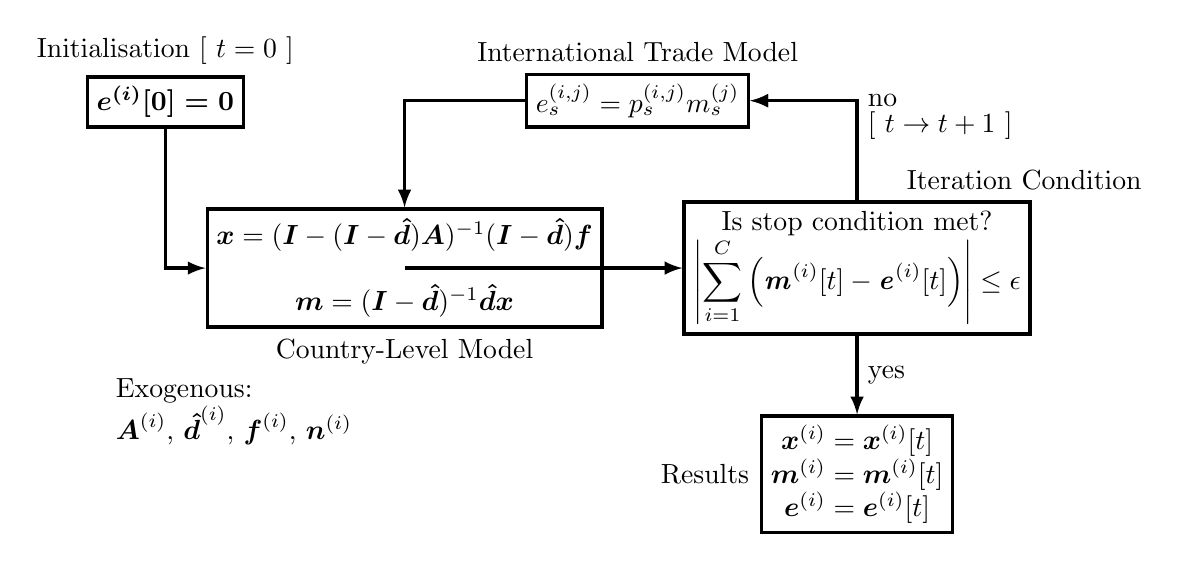
\begin{tikzpicture}[>=latex, very thick]
	\tikzstyle{all nodes}=[shape=rectangle]
	\tikzstyle{box}=[draw]
	% % Nodes
	% init
	\node[box,label=above:{Initialisation [ $t=0$ ]}](init)
	{$\boldsymbol{e^{(i)}[0] = 0}$};
	% country-level model
	\node[box, below right= and -.5cm of init, 
		  align=center, label=below:Country-Level Model]
	(country)
	{
		$
		\boldsymbol{x} = 
		(\boldsymbol{I} - 
		(\boldsymbol{I} - \boldsymbol{\hat{d}})
		\boldsymbol{A})^{-1} 
		(\boldsymbol{I} - \boldsymbol{\hat{d}})\boldsymbol{f}
		$ \\\\
		$
		\boldsymbol{m} = 
		(\boldsymbol{I} - 
		\boldsymbol{\hat{d}})^{-1} 
		\boldsymbol{\hat{d}}\boldsymbol{x}
		$
	};
	% international trade model
	\node[box, above right= and -1cm of country](trade)
	[label=above:International Trade Model]
	{
		$e_s^{(i,j)} = p_s^{(i,j)}m_s^{(j)}$
	};
	% iteration condition
	\node[box, right= of country, align=center](iteration)
	[label=60:Iteration Condition]
	{
		Is stop condition met?
		\\
		$
		\displaystyle \left| \sum^C_{i=1} \left(\textbf{\textit{m}}^{(i)}[t] -
		\textbf{\textit{e}}^{(i)}[t] \right) \right| \leq \epsilon
		$
	};
	% results
	\node[box, below=of iteration, align=center](result)
	[label=left:Results]
	{
		$\boldsymbol{x}^{(i)}=\boldsymbol{x}^{(i)}[t]$ \\
		$\boldsymbol{m}^{(i)}=\boldsymbol{m}^{(i)}[t]$ \\
		$\boldsymbol{e}^{(i)}=\boldsymbol{e}^{(i)}[t]$
	};
	% Exogenous annotation
	\node[below left=0.5cm and -2cm of country, align=left] {
	Exogenous: \\
	$\boldsymbol{A}^{(i)}$,
	$\boldsymbol{\hat{d}}^{(i)}$,
	$\boldsymbol{f}^{(i)}$,
	$\boldsymbol{n}^{(i)}$
	};
	% % Connectors
	\draw [->] (init) |- (country);
	\draw [->] (country) |- (iteration);
	\draw [->] (iteration) |- node[right]{no}(trade);
	\draw [->] (iteration) |- node[below right]{[ $t \rightarrow t+1$ ]}(trade);	
	\draw [->] (trade) -| (country);
	\draw [->] (iteration) -- node[right]{yes}(result);
\end{tikzpicture}
\caption{The model algorithm: total production, imports and exports are calculated for a given set of exogenous coefficients. Note that square brackets have been introduced to designate the iteration variable $t$, which tracks the quantities that are iteratively recalculated as the algorithm runs.}\label{fig:algorithm}
\end{figure}

Figure \ref{fig:algorithm} shows a schematic version of the algorithm for calculating imports and exports from the four groups of coefficients.
\subsubsection*{Initialisation}
All export demands are set to 0.

\subsubsection*{Country-level model}
Inside each country, total demand is calculated using the export demands (which were initially set to zero), final demands, technical coefficients and import ratios, as per \cref{eqn:xmodel}.
This step maintains the standard input-output matrix inversion.
From total demand, import demand can be calculated via the import ratios as in \cref{eqn:mmodel}.

\subsubsection*{Iteration condition}
At this point a `stop condition' is checked: does the total level of global import demand match total exports in each sector, to within some small value,  $\epsilon > 0$\footnote{More specifically, as shown in Figure \ref{fig:algorithm}, we verify that the length of the vector of differences between the global sum of all imports and the global sum of all exports for each sector does not exceed $\epsilon$. This approach ensures that global export and import totals must balance for all sectors simultaneously.}?
In the first run through the iteration, this stop condition will certainly fail, because exports have just been set to zero.

\subsubsection*{International trade model}
The import demands calculated in the country-level models can be divided up into export demands using the import propensities using to \cref{eqn:emodel}.
These new export demands replace the export demands from the previous iteration (which were all zero the first time round).
With a new set of export demands calculated the algorithm returns to the country-level model.

The iteration continues in this way, moving between the country-level and the international-level models, until the system of imports and exports converges and the stop condition is met \footnote{An analysis confirming the convergence of the algorithm is the focus of upcoming work by Anthony Korte of the UCL Department of Mathematics.}.

Solving the system algorithmically rather than relying on the standard methods of linear algebra allows for a greater flexibility in the way that the model may be extended in future work. For example, provided that care was taken to maintain its stability, the algorithmic approach could be applied even if the assumption of linear production functions were to be relaxed in order to model economies of scale.


\section{Analysis}\label{sec:analysis}
The model combining input-output country descriptions and the international trade network allows for the measurement of the total input required to make a single unit of a particular sector's product.
Since WIOD reports product flows in millions of US dollars (\$M), this will also be the unit of all the following analysis.
In all the following analysis, the model was initialised with data from 2010.

\subsection{Simple modelling approaches}
\label{sec:simple_modelling_approaches}

\subsubsection*{Economic significance}
A simple way to measure the significance to the global economy (hereafter `significance') of a particular sector in a given country is to artificially reduce final demand for the products of that country-sector by one unit, to recalculate all flows in the model based on this new final demand and to measure the response of each other sector in each other country in the model.

This is a particularly powerful means of assessing the significance of a given country-sector, because it not only takes account of the \textit{direct} effects of such a change - a reduction in the output of the sector in question and of those sectors supplying that sector's intermediate demand - but also of the full spectrum of \textit{indirect} effects, on those sectors which supplied the demand of the sectors who supplied the sector in question, on \textit{their} suppliers and so on.

We can formalise the final-demand change in sector $s$ in country $i$ as:

\begin{equation}\label{eqn:reduce_fd_by_one}
f_s^{(i)} \rightarrow f_s^{\prime (i)} \equiv (f_s^{(i)} - 1)
\end{equation}
The simplest way to define `response' is as the change of total output of all sectors, $r$, in all countries, $j$, caused by the reduction:
\begin{equation}
\Delta_{s}^{(i)} x_{r}^{(j)} \equiv (x_{r}^{\prime(j)} - x_r^{(j)})
\end{equation}
where $x_{r}^{\prime(j)}$ is the total output of sector $r$ in country $j$ after the change in \cref{eqn:reduce_fd_by_one} has taken place and the model has been recalculated according to Figure \ref{fig:algorithm}.
$\Delta_{s}^{(i)} x_{r}^{(j)}$ is thus the change in output of sector $r$ in country $j$ induced by the change in final demand for sector $s$ in country $i$.

The total response across all countries and all sectors induced by sector $s$ in country $i$ is:
\begin{equation}
\eta_s^{(i)} \equiv \Delta x_{s}^{(i)} = \sum_j \sum_r \Delta_{s}^{(i)} x_{r}^{(j)}
\end{equation}
and the average response induced by all sectors in country $i$ is:
\begin{equation}
\eta^{(i)} = \frac{\sum_s \eta_s^{(i)}}{S}
\end{equation}
where $S$ is, as before, the number of sectors in country $i$'s economy.

Sectors with a larger value of $\eta_s^{(i)}$ require a larger amount of input to produce each unit of their output. $\eta{(i)}$ can thus be thought of as a country-level significance measure, with larger values implying a economy which, on average, has a greater significance on production in the rest of the world.

Figure \ref{tbl:least_efficient_countries} shows the 10 most significant countries by this measure.
China is the world's most significant economy, a \$1M reduction in final demand leading to an average \$2.36M reduction in total output worldwide.

\begin{figure}
	\centering
	\subfigure[most significant countries]
	{
		\begin{tabular}{lr}
		\toprule
		Country & $\eta^{(i)}$\\
		\midrule
          China &       2.36 \\
 Czech Republic &       1.98 \\
       S. Korea &       1.95 \\
         Russia &       1.94 \\
       Bulgaria &       1.92 \\
          Japan &       1.90 \\
          Italy &       1.90 \\
         Poland &       1.89 \\
        Finland &       1.88 \\
       Portugal &       1.87 \\
		\bottomrule
		\end{tabular}
		\label{tbl:least_efficient_countries}
	}
	\subfigure[China's most significant sectors]
	{
		\begin{tabular}{lr}
		\toprule
		       Sector & $\eta_s^{(\text{China})}$\\
		\midrule
		     Vehicles &       2.47 \\
		         Food &       2.20 \\
		     Plastics &       2.20 \\
		       Metals &       2.17 \\
		    Machinery &       2.17 \\
		         Wood &       2.14 \\
		  Electricals &       2.13 \\
		 Construction &       2.12 \\
		     Textiles &       2.11 \\
		        Paper &       2.10 \\
		\bottomrule
		\end{tabular}
		\label{tbl:chinas_least_efficient_sectors}
	}
	\caption{Response to a \$1M reduction in final demand, in terms of difference induced in the total output, $x$, of other sectors. Only the largest 10 are shown.}
\end{figure}

This is perhaps a surprising result.
How can the US not be the most significant economy in the world?
To investigate further, it is useful to split the significance measure, $\eta^{(i)}$, into foreign and domestic effects, as follows:

\begin{align}
\eta_s^{*(i)} \equiv \Delta x_{s}^{*(i)} & = 
	\sum_{j \neq i} \sum_r \Delta_{s}^{(i)} x_{r}^{(j)} \\
\eta^{*(i)} & = 
	\frac{\sum_s \eta_s^{*(i)}}{s}
\end{align}
and
\begin{align}
\eta_s^{\dagger(i)} \equiv \Delta x_{s}^{\dagger(i)} & = 
	\sum_r \Delta x_{sr}^{(ii)} \\
\eta^{\dagger(i)} & = 
	\frac{\sum_s \eta_s^{\dagger(i)}}{s}
\end{align}
such that
\begin{equation}
\eta^{(i)} = \eta^{*(i)} + \eta^{\dagger(i)}
\end{equation}
Figure \ref{fig:countries_domestic_vs_foreign} shows how the average response across all sectors divides between domestic response, $\eta_s^{\dagger}$, and foreign response, $\eta_s^{*}$, for each country. 
An OLS regression line has been added to the plot.
All the countries lying close to the line have a similar total significance, $\eta^{(i)}$.
The region below the line is the region of less-than-average significance and that above the line is the region of greater-than-average significance.
China is immediately visible as an outlier.
Its economy is around one-third more significant ($\eta = 2.36$) than that of Brazil ($\eta = 1.75$) or India ($\eta = 1.74$), but almost all of this extra significance relates to its impact on its own domestic sectors.
Thus China's significance to the world economy shows itself largely in China itself. China is significant to the extent that it uses disproportionately large amounts of its own productive output in its production technology.
This may perhaps be evidence of the much-vaunted end of low labour costs in China  \parencite{li_end_2012, the_economist_end_2012} although further research would be needed to verify this.

\begin{figure}
\centering
%\includegraphics[width=\textwidth]{"images/country response domestic vs foreign - tweaked".pdf}
\caption{The total response of the global economy to a reduction in final demand, averaged across every sector in a country. 
`Response' is defined as the total production lost across all sectors.
Here, response has been divided into domestic, where the response is measured only in the country whose final demand has been reduced, and foreign, where the response is measured in all other countries only.
The solid line shows the result of an OLS regression, with the grey shaded area being the 5\% confidence interval.}
\label{fig:countries_domestic_vs_foreign}
\end{figure}

\subsubsection*{Economic self-reliance}
Countries further to the left of Figure \ref{fig:countries_domestic_vs_foreign}, such as Brazil, India, Japan, Russia, Turkey and the USA, are more self-reliant than those on the right, such as Luxembourg, Belgium, the Netherlands and Denmark.
This self-reliance can be made precise by measuring the ratio of domestic response to foreign response:
\begin{equation}
\phi^{(i)} = \frac{\eta^{*(i)}}{\eta^{\dagger(i)}}
\end{equation}
Figure \ref{fig:phi-vs-pop} shows the relationship between $\phi^{(i)}$ and population in 2010 (World Development Indicators, The World Bank).

The positive slope of the regression line (significant at 0.1\%) indicates that larger countries are generally more self-reliant.
Brazil and Australia are both more self-reliant than their population would suggest.
Belgium and the Netherlands are less self-reliant in the same sense.
Further research might be put into which sectors cause the largest share of these atypical self-reliance measures, particularly that of Brazil as that country is the largest outlier by a wide margin.

\begin{figure}[tb]
\centering
\includegraphics[width=\textwidth]{"images/phi vs population - tweaked".pdf}
\caption{}
\label{fig:phi-vs-pop}
\end{figure}

\subsection{A unified network approach}\label{sec:networkapproach}
The flow of products between countries can be viewed as a weighted, directed network, where countries are nodes, and the weights of each edge represents the magnitude of the flow between them \parencite{nystuen_graph_1961,serrano_topology_2003,bhattacharya_international_2008,baskaran_heckscher-ohlin_2011}.
Similarly with the sector-sector flows which constitute an input-output model \parencite{blochl_vertex_2011,fedriani_simplifying_2012}.
Network science has developed useful ways to analyse the sort of weighted, directed networks which the constitute the present model, but a single network representation is required which combines the international and the sub-national networks.

Recall from section \ref{sec:importratios} above, that products arriving at the shores of an importing country are put into a warehouse along with domestically produced products, at which point the two become indistinguishable.
If an additional assumption is made that domestic sectors take from this warehouse by means of a random sample, then the fraction of products in each sample from abroad will be identical, as will the fraction of imported products from each exporter.
These fractions will be set by the import ratios and import propensities respectively.

This additional assumption allows us to specify a complete system of intermediate (input-output) flows, $y_{rs}^{(i,j)}$, from sector $r$ in country $i$ to sector $s$ in country $j$, thereby effectively reconstructing the WIOT which was diverted from in section \ref{sec:algorithm}:

\begin{equation}\label{eqn:y_rsij}
y_{rs}^{(i,j)} = p_{r}^{(i,j)} d_{r}^{(j)} a_{rs}^{(j)} x_{s}^{(j)}
\end{equation}
\Cref{eqn:y_rsij} can be understood as follows:
sector $s$ in country $j$ requires an amount $a_{rs}^{(j)} x_{s}^{(j)}$ of sector $r$'s product to produce its total output;
a fraction $d_{r}^{(j)}$ of this will be supplied by imports;
a fraction $p_{r}^{(i,j)}$ of these imports will come from country $i$. Note that since countries do not import their own exports, $p_s^{(i,i)}=0,\ \forall i$, and the expression holds trivially for $i=j$.

The fractions of each type of demand for $s$ in country $j$ which was exported by country $i$ are given by similar expressions:

\begin{subequations}
\begin{equation}\label{eqn:f_sij}
f_{s}^{(i,j)} = p_{s}^{(i,j)} d_{s}^{(j)} f_{s}^{(j)}
\end{equation}
\begin{equation}\label{eqn:e_sij}
e_{s}^{(i,j)} = p_{s}^{(i,j)} d_{s}^{(j)} e_{s}^{(j)}
\end{equation}
\begin{equation}\label{eqn:n_sij}
n_{s}^{(i,j)} = p_{s}^{(i,j)} d_{s}^{(j)} n_{s}^{(j)}
\end{equation}
\end{subequations}
where, as previously, $f$ is final demand, $e$ is export demand and $n$ are investments.

Along with the sector-to-sector flows given by \cref{eqn:z_dagger_and_star}, this allows for the representation of all the flows in the present model as a single network, to which standard network analysis techniques can then be applied.

\begin{figure}[tb]
\centering
\includegraphics[width=\textwidth]{"images/Chinese Vehicles Top 10 Countries".png}
\caption{A network representation of the seven most-affected countries following a reduction in final demand for the Chinese vehicles sector. Node size is proportional to eigenvector centrality, and edge width is proportional to the change in flow.}\label{fig:chnvehtop6}
\end{figure}

This reformulation demonstrates the connection between the model described in this paper and the established world input-output table approach, allowing us to visualise the individual country-sector to country-sector flows (or changes in such flows) for any model scenario, such as that calculated in section \ref{sec:simple_modelling_approaches} in response to a reduction of demand in China for the Vehicles sector by \$1M.

The change to every such flow (both $y_{rs}^{(i,j)}$ and $z_{rs}^{(i)}$ type flows) in the eight most-affected countries is recorded and visualised in figure \ref{fig:chnvehtop6}.
Node size is proportional to eigenvector centrality and the edge weight is proportional to the change induced in the particular flow be the reduction in final demand.
This diagram reveals the patterns and shapes of the various economies which would be hard to pick out in the raw flow matrix.

\subsection{Comparison with a world input-output table}
As discussed in section \ref{sec:litreview}, the modelling approach presented here relaxes the rigidity of the world input-ouput table's assumptions about the patterns of global trade.
In so doing, it also reduces the amount of data required to estimate the place in the world of countries which are not covered by WIOD.
But since the present iteration of the model can be made equivalent to a WIOT (as shown in section \ref{sec:networkapproach}), any of the analyses presented here could equally well be performed using the world input-output table directly.
It is therefore important to verify that the model in its present, most simple form, behaves similarly to a WIOT before any further development is done.

To this end, the results of the experiment of section \ref{sec:simple_modelling_approaches}, reducing demand for Chinese vehicles, is repeated using a WIOT, and the results are compared in figure \ref{fig:chn_vec_model_vs_wiot}.

The response to a reduction in demand for Chinese vehicles is summed over sectors in each country.
The countries are then ranked according to the size of the response.
The ranks produced by the WIOT are shown on the left-hand side, and those produced by the present model on the right.
Visually, the results seem broadly comparable and have a Spearman rank correlation coefficient \parencite{spearman_proof_1904} of 0.96.
This gives some confidence in concluding that this first, simplest iteration of the model behaves in a similar fashion to the WIOT it seeks to extend.

\begin{figure}[p]
\centering
\includegraphics[height=0.8\textheight]{"images/chn_vec_rank_change_wiot_vs_model".pdf}
\caption{A comparison of the results of the Chinese vehicle experiment performed on a WIOT (on the left) and on the present model (on the right).
Vertical position represents the rank of the country in terms of how affected it is by a reduction in demand for Chinese vehicles.\\
\textsuperscript{*}Taiwan is ranked last in the present model.
This is because the UN provides no trade data for the territory.
All Taiwan's import ratios are therefore zero (i.e. Taiwan is modelled as being entirely self-sufficient.)}
\label{fig:chn_vec_model_vs_wiot}
\end{figure}


\section{Conclusions}\label{sec:conclusions}
In this paper, a new model of global trade has been presented, combining two distinct modelling approaches for the internal workings of national economies and for international trade.
The model incorporates information from two extremely extensive data sets, the UN COMTRADE database and the World Input-Output Database, giving it a level of real world economic detail exceeding that of almost all previous work.

The model equations are solved iteratively, thus avoiding the limitations and assumptions of the traditional world input-output table approach which are no longer necessary in this age of very fast computing, and lending the model the flexibility to accommodate a wide variety of possible extensions, such as the consideration of non-linear production functions, limited production capacities and non-clearing markets.
It also offers a rich set of coefficients to examine and manipulate, with the addition of import ratios and import propensities to the traditional approach of national input-output models, which will facilitate its integration with other social science models, such as those that model how countries choose to trade with one another.

The model allows for the definition and analysis of a powerful new measure of the global economic significance of each sector within a national economy, gauging the degree to which that sector drives economic activity across the world. In initial investigations, China was found to be a considerable outlier in terms of its economic significance, driven by high consumption of its own domestically produced products and services. Following this analysis, a measure of economic self-reliance was introduced, which was was found to vary inversely with population. These results represent preliminary analyses only, with far more scope for detailed investigation of international trade patterns and alternative global economic scenarios now that the model is operational.

Finally, a method is presented to transform the structure of the model into that of a traditional world input-output table, allowing for the deployment of the tools and analyses of the network science literature. A very simple example of this approach was presented, with further analyses to follow in future work.

Further work on the model will include the relaxation of the traditional input-output assumptions, beginning with the introduction limits on production capacity, with the goal of creating a fully dynamic version of the model to analyse the change in trade patterns over time. Ultimately, the model will also be combined with further submodels representing migration, international security and the distribution of development aid, to create a fully integrated representation of these global processes.






\section*{Acknowledgements}

The authors acknowledge the financial support of the UK Engineering and Physical Sciences Research Council (EPSRC) under the grant ENFOLDing -- Explaining, Modelling, and Forecasting Global Dynamics, reference EP/H02185X/1. 

%The authors would also like to thank the anonymous reviewers, whose constructive comments contributed significantly to the final version of this article.


\printbibliography

\end{document} 
